\documentclass[varwidth=true, border=2pt]{standalone}

\usepackage{pgfplots}
\usepackage{tikz}

\usetikzlibrary{calc,patterns,angles,quotes}

\begin{document}
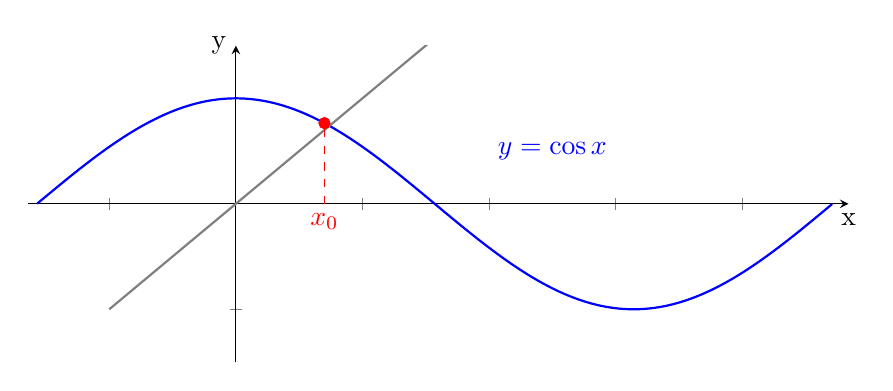
\begin{tikzpicture}
    \begin{axis}[
        legend pos=south east,
        axis x line=middle,
        axis y line=middle,
	every axis x label/.style={at={(current axis.right of origin)},anchor=north},
	every axis y label/.style={at={(current axis.above origin)},anchor=east},
	xticklabels=\empty,
	yticklabels=\empty
        grid = none,
        width=12cm,
        height=5.6cm,
        grid style={dashed, gray!1},
        xmin=-1.1,     % start the diagram at this x-coordinate
        xmax= 4.3,    % end   the diagram at this x-coordinate
        ymin=-1.25,     % start the diagram at this y-coordinate
        ymax= 1.25,   % end   the diagram at this y-coordinate
        xlabel=x,
        ylabel=y,
        enlargelimits=true,
        tension=0.08]

        \addplot[domain=-1.57:4.71,blue, thick,samples=250] {cos(deg(x))};
        \addplot[domain=-1:2, gray, thick,samples=250] {x};


	\addplot[dashed,red,mark=none] coordinates{(0.7,0)(0.7,0.765)} node[below, pos=0] {$x_0$}; %x0
	\addplot[red, only marks, mark=*] coordinates {(0.7,0.765)};
	\node(x1)[blue] at (axis cs: 2.5,0.5){{$y = \cos x  $}};
    \end{axis}
\end{tikzpicture}





\end{document}